\renewcommand{\thesection}{S\arabic{section}}
\renewcommand{\thefigure}{S\arabic{figure}}
\renewcommand{\thetable}{S\arabic{table}}
\setcounter{section}{0}
\setcounter{figure}{0}
\setcounter{table}{0}

\section*{MULTIMODAL ATTENTION-BASED DEEP LEARNING FOR ALZHEIMER'S DISEASE DIAGNOSIS}

\section*{Supplementary Material}
\label{section:supp-materials}


\section{Genetic Data Pre-processing}
\label{section:genetic}
The genetic data consists of the whole genome sequencing (WGS) data from 805 ADNI participants by Illumina’s non-Clinical Laboratory Improvement Amendments (non-CLIA) laboratory at roughly 30–40 × coverage in 2012 and 2013. The resulting variant call files (VCFs) have been generated by ADNI using Broad best practices (Burrows-Wheeler Aligner (BWA) and Genome Analysis Toolkit (GATK)-haplotype caller) in 2014. We first filtered the SNPs by the Hardy-Weinberg equilibrium (HWE) test for each site (p-values) by removing SNPs with HWE p $<$ 0.05. We then checked the genotype quality (GQ) and removed SNPs with GQ $<$ 20. Next, we filtered by minor allele frequency (MAF) and removed sites with MAF $<$ 0.01. Lastly, we performed genotype value filtering where we excluded sites based on the proportion of missing data and removed sites with a missing rate $>$ 0.05. After filtering with the above criteria, we utilized genes known to be related to Alzheimer’s Disease. In this step, we first downloaded a list of all AD-related genes from the AlzGene Database (\url{http://www.alzgene.org/}), which contains 680 genes in total. Then we searched these genes in the UCSC genome browser (\url{https://genome.ucsc.edu/}) and kept the 640 genes that matched NCBI RefSeq annotation. We extracted these gene regions from RefSeq Annotation (gff file) in Bed format and use them to filter the SNPs further. We only retain the genes that are located in these regions. After selecting the 680 genes of known association with AD, we had 547,863 SNPs left. As discussed in the {\hyperref[subsubsection:genetic_proc]{Genetic Data Pre-processing} Section}, we needed to find a way to reduce the number of features. We used a Random Forest Classifier to create a list of the most important features. Since this is a supervised method of creating features, this brought more promising results to the performance, in contrast to an approach such as principal component analysis (PCA) which is unsupervised. To find the best set of features, we tried using 50, 100, 150, and 200 forests as the parameter in the classifier. After creating the four sets of features, we used a validation set (10\% from the training) to do hyperparameter tuning (as described in \ref{section:hyper}), for each set of features, we found that the set from 100 forests performed the best on the validation set resulting in the accuracy described in {the \hyperref[subsection:uni_frame]{Performance of Unimodal Models} Section}. 

\section{Clinical Features}
\label{section:clinical}
In the {\hyperref[subsection:robust]{Model Robustness} Section} we discussed the value of clinical features to the model's performance. To ensure that there are no variables in the data that could potentially give an unfair advantage to the model (e.g.\ medication that a patient takes, only when they already have AD), we carefully examined all available variables. We fit a Random Forest classifier (from the scikit-learn package \cite{sklearn_api}) which outputs the features along with their importance score. The importance of a feature is computed as the (normalized) total reduction of the criterion brought by that feature \cite{sklearn_api}. Figure \ref{fig:clinical_imp} shows the full list of features and their importance. 

\begin{figure}[H]
\begin{center}
    \caption{\textbf{Clinical feature importance.} The graph shows all the clinical features used in our model in order of most important to least important}
    \label{fig:clinical_imp}
  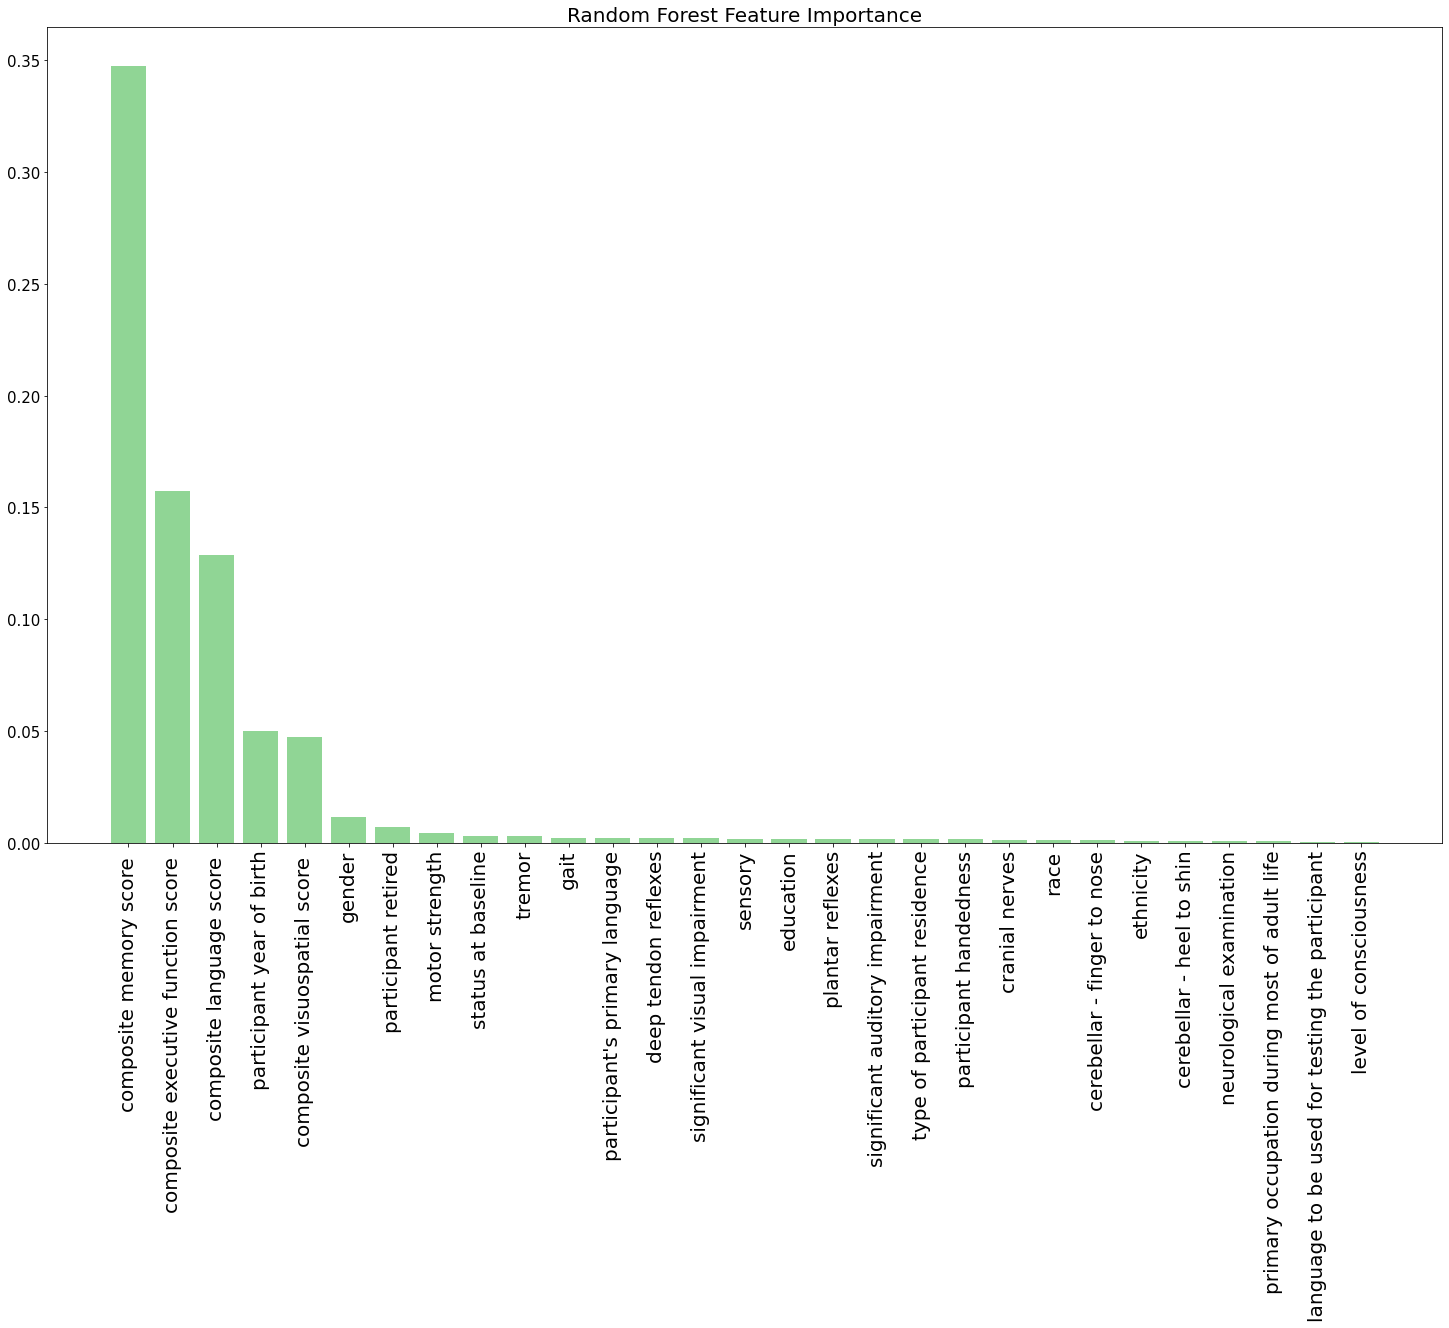
\includegraphics[scale=0.3]{figures/importance.png}
  \end{center}
\end{figure}

\newpage
\section{Imaging Data Pre-processing}
\label{section:img_preproc}
The images used for our study are pre-processed by ADNI with specific image correction steps:
\begin{enumerate}
\item Gradwarp: gradwarp is a system-specific correction of image geometry distortion due to gradient non-linearity. The degree to which images are distorted due to gradient non-linearity varies with each specific gradient model. We anticipate that most users will prefer to use images which have been corrected for gradient non-linearity distortion in analyses.
\item B1 non-uniformity: this correction procedure employs the B1 calibration scans noted in the protocol above to correct the image intensity non-uniformity that results when RF transmission is performed with a more uniform body coil while reception is performed with a less uniform head coil.
\item N3: N3 is a histogram peak sharpening algorithm that is applied to all images. It is applied after grad warp and after B1 correction for systems on which these two correction steps are performed. N3 will reduce intensity non-uniformity due to the wave or the dielectric effect at 3T. 1.5T scans also undergo N3 processing to reduce residual intensity non-uniformity.
\end{enumerate}
We followed the same pre-processing steps as Bucholc et al. \cite{BUCHOLC2019157}, El-Sappagh et al. \cite{ELSAPPAGH2020197}, and Abuhmad et al. \cite{ABUHMED2021106688}, which relied on ADNI’s correction steps without further modification.
\newline 
To demonstrate that the performance of the unimodal imaging model is not significantly impacted by the addition of more brain slices, we report the optimized performance of the model with just the middle three slices, 2 more images per angle (6 more in total), 5 more images per angle, 10 more images per angle, 20 more images per angle, and 50 more images per angle. We report both F1-Scores and accuracy (averaged across 3-fold validation set), which follow a similar trend shown in \ref{fig:mri_exp}. The difference in performance between no additional slices (used in the paper) and 20 additional slices are all within 1 percent. When adding 50 slices to each angle, we observe a significant decline in performance. Thus, we proceeded with the original choice of just using the middle of the brain.  

\begin{figure}[H]
\begin{center}
    \caption{\textbf{Validation F1-Score and Accuracy Trend as Number of Images Increases.} The graph shows that the unimodal imaging model does not significantly benefit from the addition of more images.}
    \label{fig:mri_exp}
  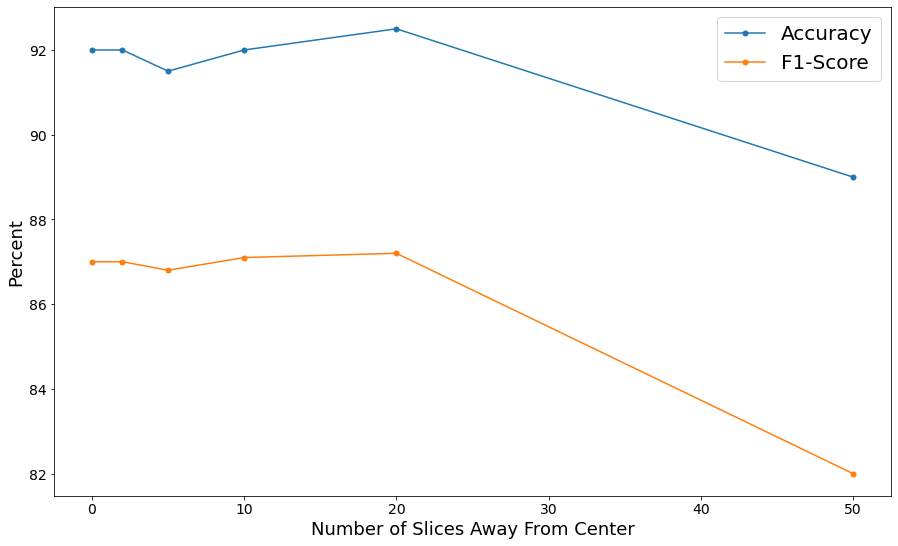
\includegraphics[scale=0.3]{figures/mri_exp.png}
  \end{center}
\end{figure}

\newpage
\noindent The decline in performance can be attributed to the fact that the slices further away from the center do not contain meaningful information and add noise to the model. The example below shows the middle three slices, followed by the outer 10 slices and outer most slices. 

\begin{figure}[H]
\begin{center}
    \caption{\textbf{Example of MRI slices as distance increases from the center.}}
    \label{fig:mri_slices}
  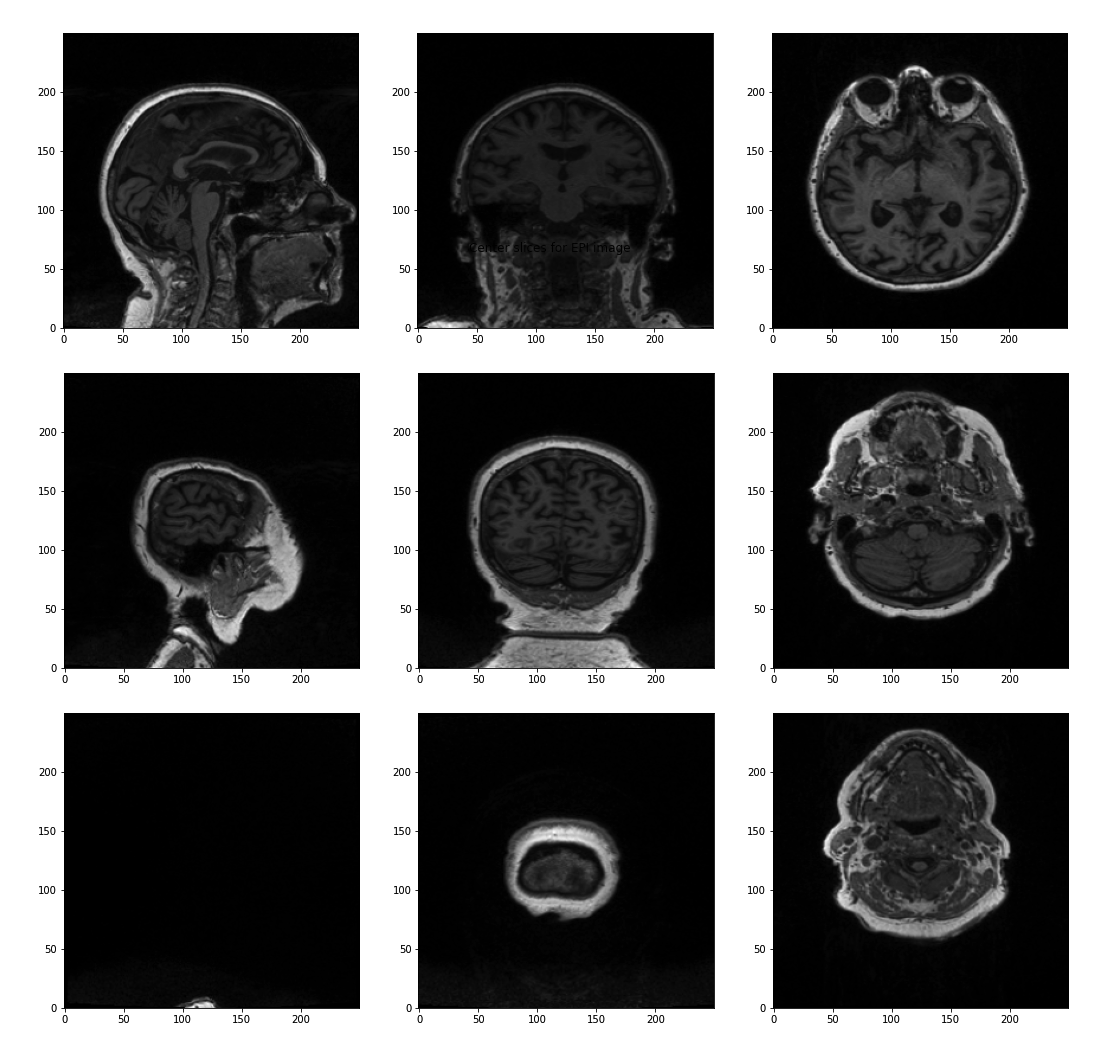
\includegraphics[scale=0.3]{figures/mri_slices.png}
  \end{center}
\end{figure}
  

\newpage
\section{Hyperparameter Tuning Methods}
\label{section:hyper}
To perform hyperparameter tuning for both unimodal and multimodal results, we randomly split the data into a training set (90\%) and a testing set (10\%). The testing set was set aside and withheld from tuning. We picked the best hyperparameters on the average validation accuracy of the 3-fold cross-validation scheme. For either a fully connected neural network or a convolutional neural network, the architecture, batch size, number of epochs, and learning rate were chosen via tuning. Table \ref{tab:hyper} describes all hyperparameters considered. 

\begin{table}[H]
\centering
\caption{\textbf{Hyperparameter Grid}}\label{tab:hyper}
\begin{tabular}{|l|l|}
\hline
\textbf{Hyperparameters} & \textbf{Values}                     \\ \hline
Learning Rate            & [0.00001, 0.1]                       \\ \hline
Dropout Values           & \{0.1, 0.2, 0.3, 0.4, 0.5\}      \\ \hline
Number of Layers         & [1, 6]                               \\ \hline
Batch Size               & \{16, 32, 64, 128\}               \\ \hline
Number of Epochs         & \{10, 20, 50, 80, 100, 150, 200\} \\ \hline
\end{tabular}
\end{table}

\noindent The hyperparameters that gave the highest accuracy for each type of model are shown in \ref{tab:best_hyper}. For the multimodal framework, the best unimodal neural network values were added into the architecture. 

\begin{table}[H]
\centering
\caption{\textbf{Best Hyperparameters}}\label{tab:best_hyper}
\begin{tabular}{|l|l|l|l|l|l|}
\hline
                  & \textbf{Learning Rate} & \textbf{Batch Size} & \textbf{Number of Layers} & \textbf{Dropout Value} & \textbf{Number of Epochs} \\ \hline
Unimodal Clinical & 0.0001                 & 32                  & 3                         & \{0.2, 0.3, 0.5\}      & 100                       \\ \hline
Unimodal Genetic  & 0.001                  & 32                  & 3                         & \{0.3,0.5\}            & 50                        \\ \hline
Unimodal Imaging  & 0.001                  & 32                  & 3                         & \{0.3,0.5\}            & 50                        \\ \hline
Multimodal        & 0.001                  & 32                  & \{3, 3, 3\}               & \{0.2, 0.3, 0.5\}      & 50                        \\ \hline

\end{tabular}
\end{table}


\section{Evaluation Metrics}
\label{eval_formula}
For our multi-class setting, we used the formulas below for each class. For example, for class 0 (control), we calculated the number of true positives, true negatives, false positives, and false negatives just for class 0. Then, we use “macro” averaged F1-score using the arithmetic mean of all the per-class F1-scores.

\begin{gather*}
Accuracy = \frac{TP+TN}{TP+TN+FP+FN}\\
Precision = \frac{TP}{TP+FP}\\
Recall = \frac{TP}{TP+FN}\\
F1 = \frac{2*Precision*Recall}{Precision+Recall} = \frac{2*TP}{2*TP+FP+FN}\\
\end{gather*}

\newpage
\section{Performance of Unimodal Models}
\label{eval_unimodal}
Table \ref{tab:uni} shows the numeric information presented in Figure \ref{fig:uni}. We report all four evaluation metrics for the best
neural network model for each modality - imaging, clinical, and genetic. The imaging model gives the best
performance overall, whereas the genetic modality gives the lowest performance. 

\begin{table}[H]
\caption{\textbf{Results of Unimodal Models.}}\label{tab:uni}
\centering
\begin{tabular}{|l|l|l|l|l|}
\hline
\textbf{} & \textbf{Accuracy (\%)} & \textbf{Precision (\%)} & \textbf{Recall (\%)} & \textbf{F1-Score (\%)} \\ \hline
Clinical  & 80.59             & 80.56              & 80.48           & 80.47             \\ \hline
Imaging   & 92.23             & 94.02              & 90.4            & 91.83             \\ \hline
Genetic   & 77.78             & 78.37              & 76.92           & 77.24             \\ \hline
\end{tabular}
\end{table}


\section{Model Robustness}
\label{tab_boxplot}
Table \ref{tab:attention} shows the numeric information presented in Figure \ref{fig:attention}.

\begin{table}[H]
\caption{\textbf{F1-Score Distribution for different attention-based and attention-free baselines.} The table shows the F1-score distribution across 100 random seeds to show the value of attention in a deep learning model. The table demonstrates that the combination of self-attention with cross-modal attention performs the best with the most narrow variation.} \label{tab:attention}
\scalebox{0.9}{%
\begin{tabular}{|l|l|l|l|l|l|}
\hline
& \textbf{Lower Whisker} & \textbf{Lower Quartile} & \textbf{Median} & \textbf{Upper Quartile} & \textbf{Upper Whisker} \\ \hline
Self-Att + Cross-Modal Att & 0.7767                 & 0.8268                  & 0.8799          & 0.9238                  & 1                      \\ \hline
Cross-Modal Att            & 0.4068                 & 0.6491                  & 0.7657          & 0.8268                  & 1                      \\ \hline
Self-Att                   & 0.7175                 & 0.8148                  & 0.8682          & 0.8799                  & 0.9238                 \\ \hline
No Attention               & 0.6396                 & 0.7714                  & 0.8148          & 0.8799                  & 0.9238                 \\ \hline
\end{tabular}}
\end{table}

\newpage
\section{Investigating Individual Class Performance}
\label{confusion}
We include confusion matrices for each of the 5 random initializations to supplement Table \ref{tab:classes} in the \hyperref[subsection:robust]{Model Robustness} Section. Each confusion matrix represents the results of our best multimodal model with respect to a random seed. 

\begin{figure}[H]

    \subfloat[Random Seed 1]{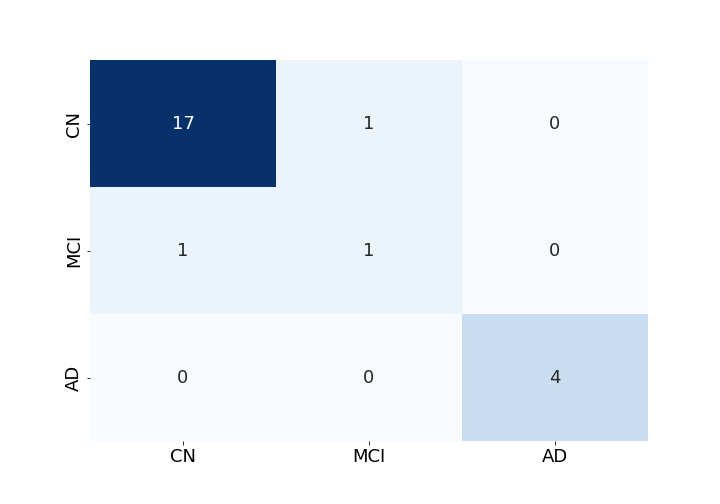
\includegraphics[width = 3in]{Multi-Modal Alzheimer's_JAMIA/figures/confusion_0.png}} 
    \subfloat[Random Seed 2]{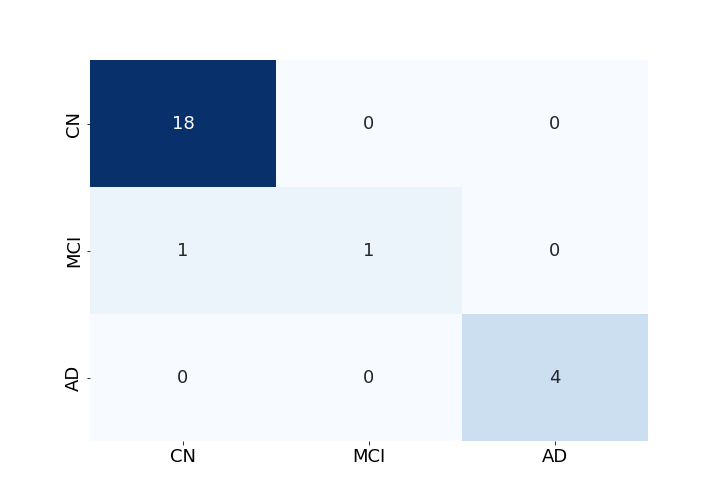
\includegraphics[width = 3in]{Multi-Modal Alzheimer's_JAMIA/figures/confusion_1.png}}\\
    \subfloat[Random Seed 3]{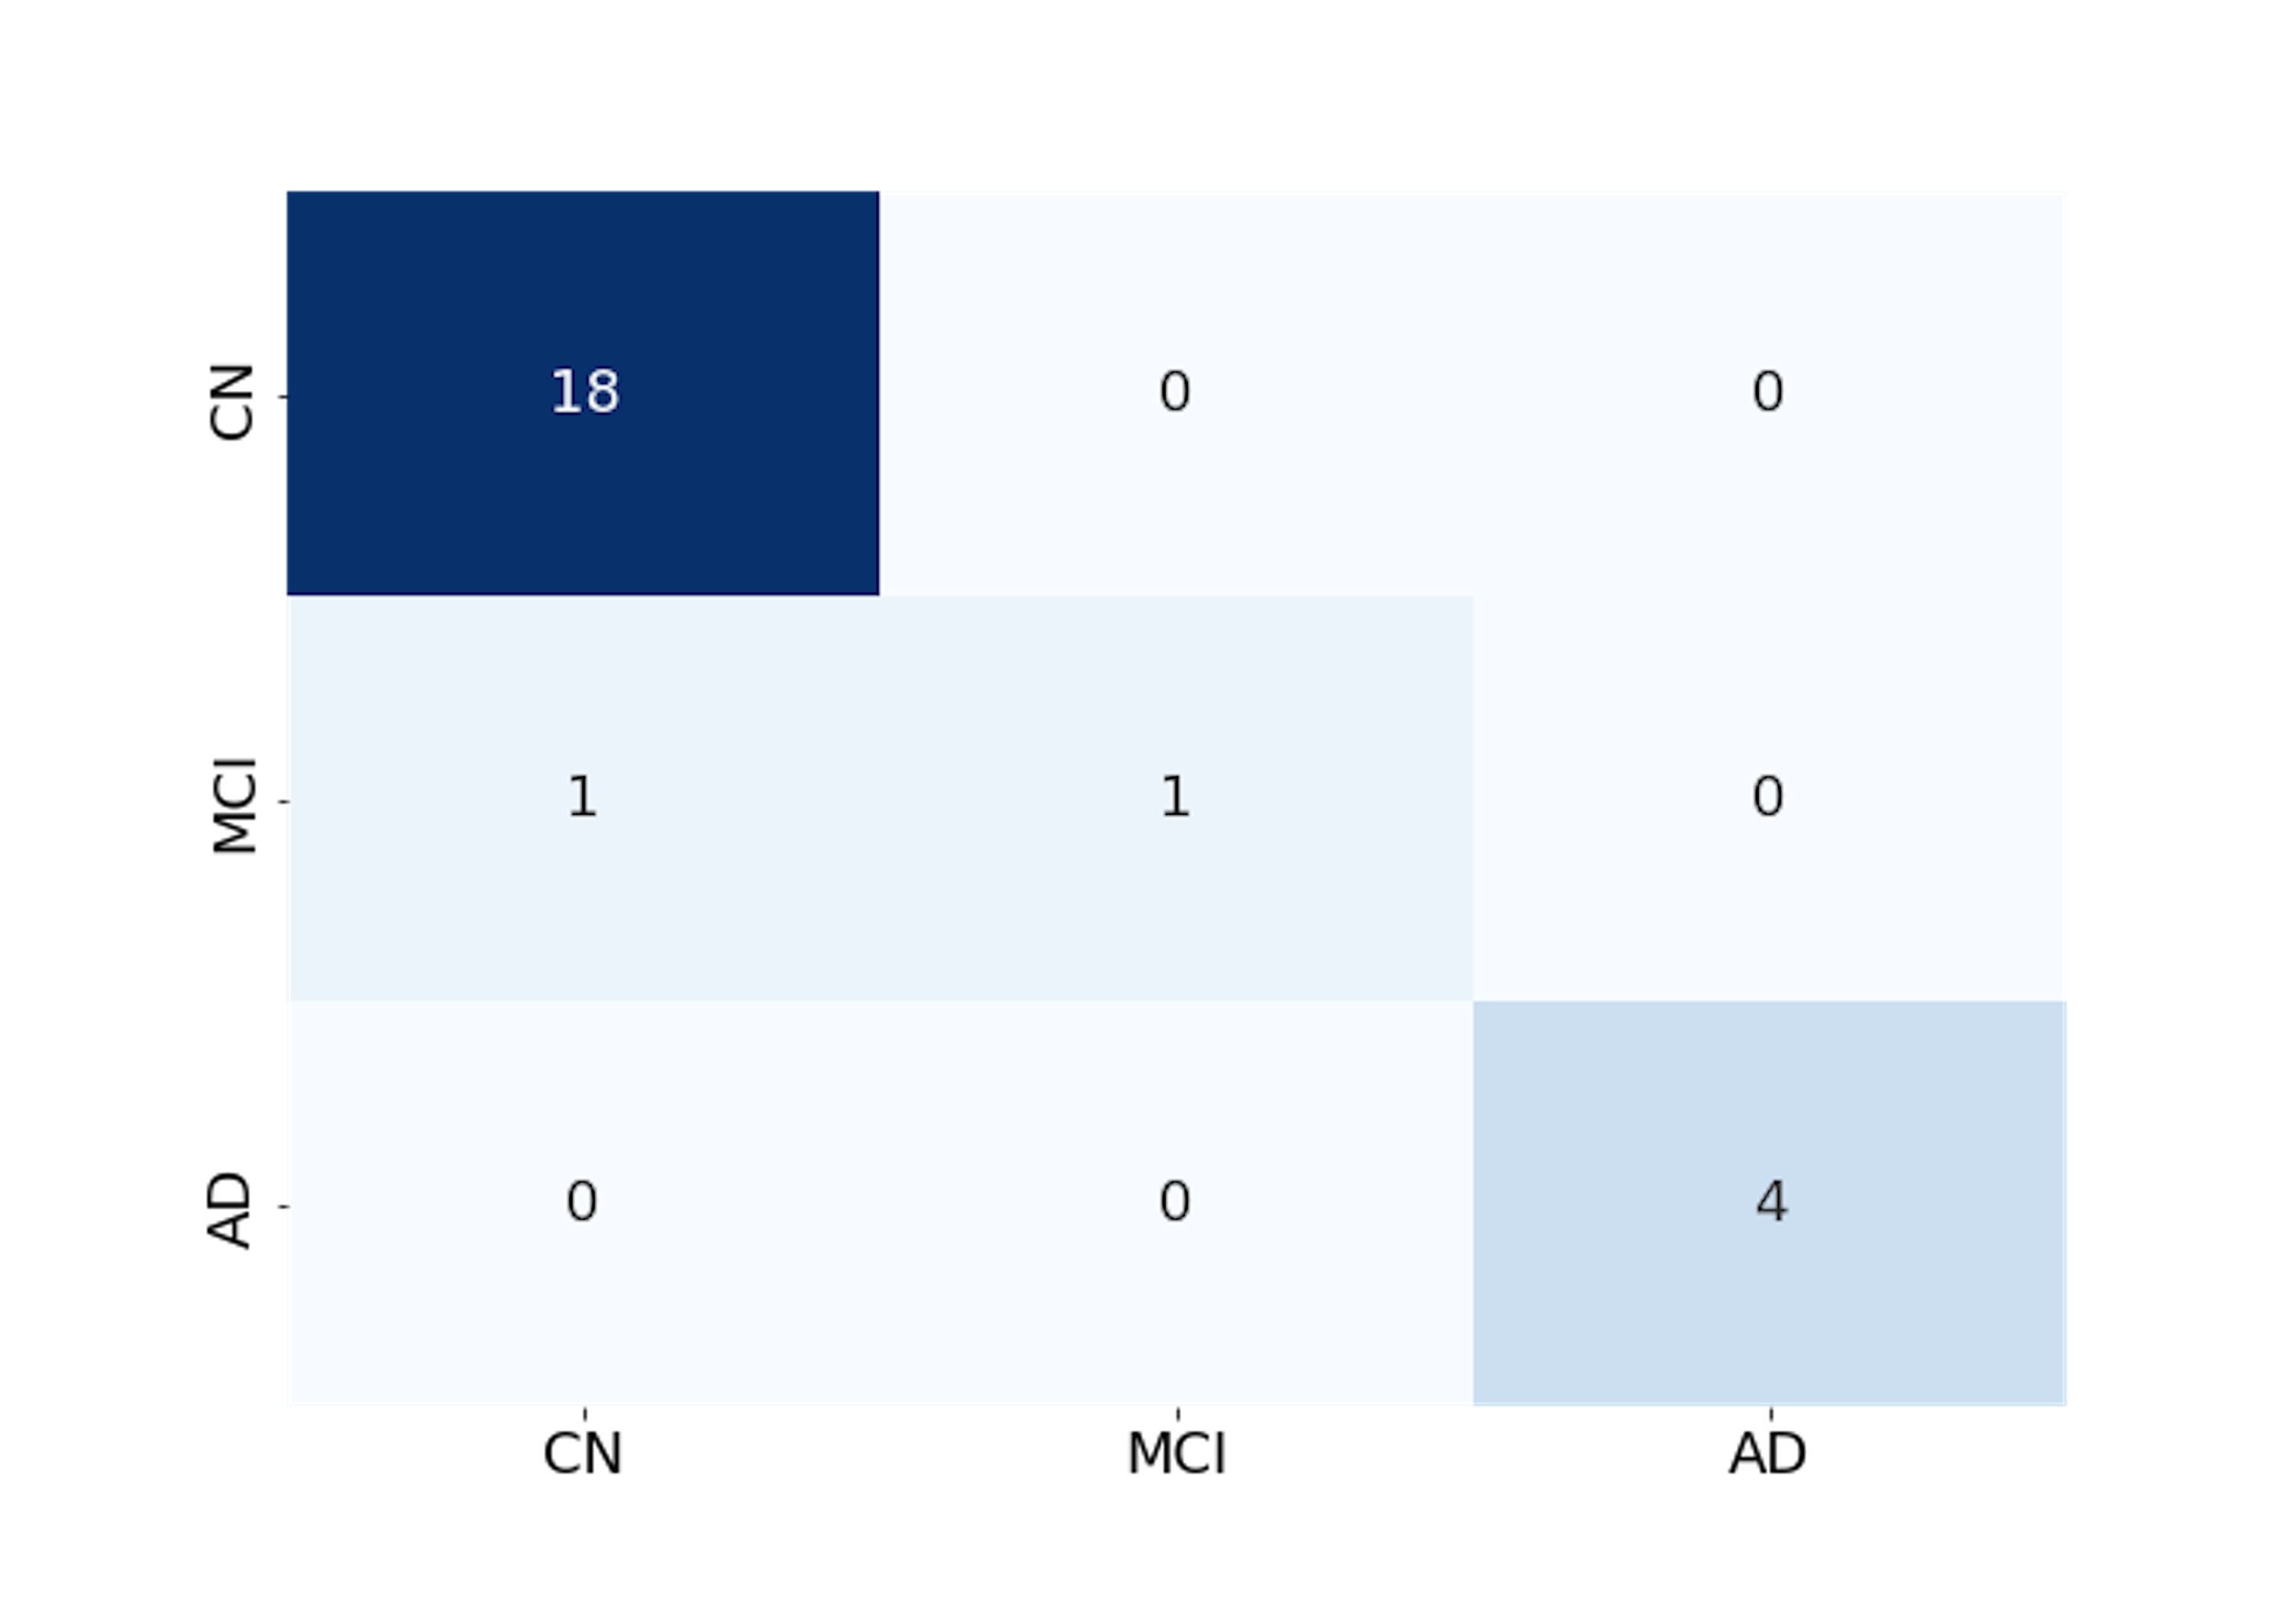
\includegraphics[width = 3in]{Multi-Modal Alzheimer's_JAMIA/figures/confusion_2.png}}
    \subfloat[Random Seed 4]{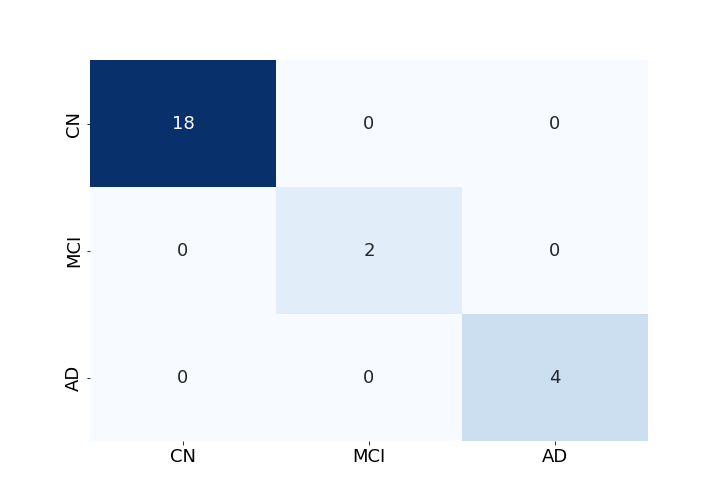
\includegraphics[width = 3in]{Multi-Modal Alzheimer's_JAMIA/figures/confusion_3.png}} \\
    \subfloat[Random Seed 5]{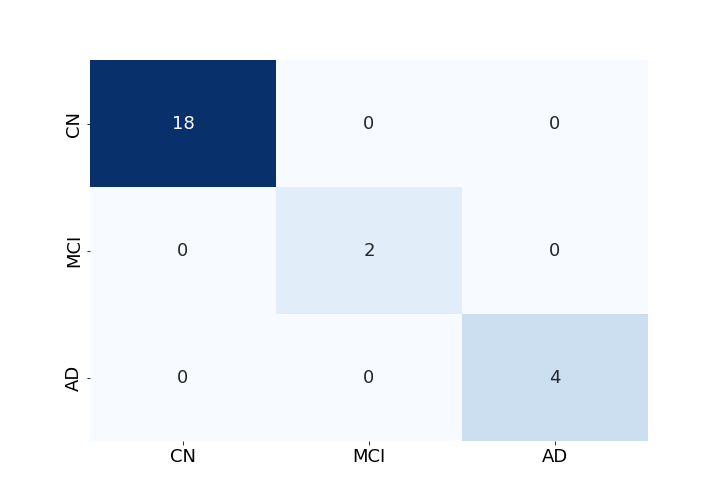
\includegraphics[width = 3in]{Multi-Modal Alzheimer's_JAMIA/figures/confusion_4.png}}
    \caption{\textbf{Confsion matricies for 5 random initializations of MADDi.}}
    \label{fig:confusion}

\end{figure}




\section{Sample Selection}
\label{section:samp_sel}
To demonstrate that our sample selection process was thorough, we show in Table \ref{tab:cross_val} the results of the models described in {\hyperref[subsection:robust]{Model Robustness} Section} on the 3-fold cross validation scheme. The metrics in the table are averaged across 5 random initializations. Since these results are similar to the ones reported on the test set in Table \ref{tab:comparison}, we consider the test set a fair sample of our data. 

\begin{table}[H]
\caption{\textbf{Cross-Validation Results}}\label{tab:cross_val}
\begin{tabular}{|l|l|l|l|}
\hline
                           & \textbf{F1-Score Val Set 1} & \textbf{F1-Score Val Set 2} & \textbf{F1-Score Val Set 3} \\ \hline
Cross-Modal Att + Self-Att & 89.74\%                     & 97.44\%                     & 92.30\%                     \\ \hline
Cross-Modal                & 87.18\%                     & 91.02\%                     & 88.46\%                     \\ \hline
Self-Att                   & 76.92\%                     & 85.89\%                     & 83.34\%                     \\ \hline
No Attention               & 79.48\%                     & 89.74\%                     & 87.17\%                     \\ \hline
\end{tabular}
\end{table}

\section{Evaluation of Modality Importance}
\label{section:modality_importance}
Table \ref{tab:modal_imp} shows the contribution and performance of each modality on the overlap patient set. The metrics were calculated as an average of five random initializations on a held-out test set. It captures the same information as Figure \ref{fig:eval_metric} in the {\hyperref[subsection:eval_imp]{Modality Importance} Section} but provides all the numeric results. 

\begin{table}[H]
\caption{\textbf{Evaluation of Modality Importance}}\label{tab:modal_imp}
\begin{tabular}{|l|l|l|l|l|}
\hline
                           & Accuracy (\%)     & Precision (\%)    & Recall (\%)       & F1-Score (\%)     \\ \hline
Clinical                   & 82.29\ { \scriptsize $\pm$ }  9.49\ & 78.92\ { \scriptsize $\pm$ } 3.68\  & 88.43\ { \scriptsize $\pm$ }  5.29\ & 78.30\ { \scriptsize $\pm$ }  6.70  \\ \hline
Genetic                    & 77.78\ { \scriptsize $\pm$ }  3.91\ & 78.37\ { \scriptsize $\pm$ }  4.64\ & 76.92\ { \scriptsize $\pm$ }  3.78\ & 77.24\ { \scriptsize $\pm$ }  4.03   \\ \hline
Imaging                    & 71.66\ { \scriptsize $\pm$ }  4.68   & 53.38\ { \scriptsize $\pm$ }  9.55\ & 62.03\ {\scriptsize $\pm$ }  9.77\ & 55.46\ { \scriptsize $\pm$ }  8.86\ \\ \hline
Clinical and Genetic       & 92.50\ { \scriptsize $\pm$ }  3.18\  & 87.05\ { \scriptsize $\pm$ }  9.36\ & 81.85\ { \scriptsize $\pm$ }  1.36\ & 83.21\ { \scriptsize $\pm$ }  4.21   \\ \hline
Genetic and Imaging        & 78.33\ { \scriptsize $\pm$ }  1.86\ & 50.88\ { \scriptsize $\pm$ }  8.19   & 52.59\ { \scriptsize $\pm$ }  6.88   & 50.07\ { \scriptsize $\pm$ }  4.28   \\ \hline
Imaging and Clinical       & 85.83\ { \scriptsize $\pm$ }  10.73  & 80.81\ { \scriptsize $\pm$ }  8.56   & 88.15\ { \scriptsize $\pm$ }  15.52  & 80.52\ { \scriptsize $\pm$ }  13.34  \\ \hline

\textbf{Clinical, Genetic, Imaging} & \textbf{96.88\ { \scriptsize $\pm$ }  3.33   }& \textbf{88.15\ { \scriptsize $\pm$ }  14.22}  & \textbf{91.23\ {\scriptsize $\pm$ }  13.37}  & \textbf{89.32\ { \scriptsize $\pm$ }  15.59 } \\ \hline
\end{tabular}
\end{table}